\chapter{Elektrochemische cellen en elektrolyse}\label{ch:g12:cells-and-electrolysis}

Een telefoon staat op een winteravond op 1 \% en valt uit. Een nacht aan
de lader, en 's ochtends is hij weer vol. In zijn \omterm{def:g12:cells-and-electrolysis:electrolysis}{accu} verloopt overdag
dezelfde \omterm{def:g7:chemical-reactions:reaction}{chemische reactie} de ene kant op, waarbij elektrische energie
vrijkomt, en 's nachts wordt ze door de lader de andere kant op
gedreven. Een \omterm{def:g11:redox:reaction}{redoxreactie} wordt een bron van elektriciteit als je haar
\omterm{def:g9:inside-the-atom:nucleus}{elektronen} door een draad laat lopen; en elektriciteit die door een
oplossing wordt gestuurd, kan een \omterm{def:g11:redox:reaction}{redoxreactie} afdwingen die uit zichzelf
nooit zou verlopen.

\begin{recall}
\omterm{def:g11:redox:oxidant}{Oxidatoren} nemen \omterm{def:g9:inside-the-atom:nucleus}{elektronen} op, \omterm{def:g11:redox:oxidant}{reductoren} staan ze af; \omterm{def:g11:redox:couple}{halfreacties},
\omterm{def:g11:redox:couple}{redoxkoppels} en \omterm{def:g11:redox:reaction}{redoxreacties} (\cref{ch:g11:redox}). Een systeem
verandert tot $Q = K$ (\cref{ch:g12:equilibrium}). Oplossingen van \omterm{def:g9:ions:ion}{ionen}
geleiden (\cref{ch:g9:ions}); de \omterm{def:g10:the-mole:amount}{mol} en de \omterm{def:g10:the-mole:avogadro}{constante van Avogadro}
(\cref{ch:g10:the-mole}).
\end{recall}

\begin{omfigure}
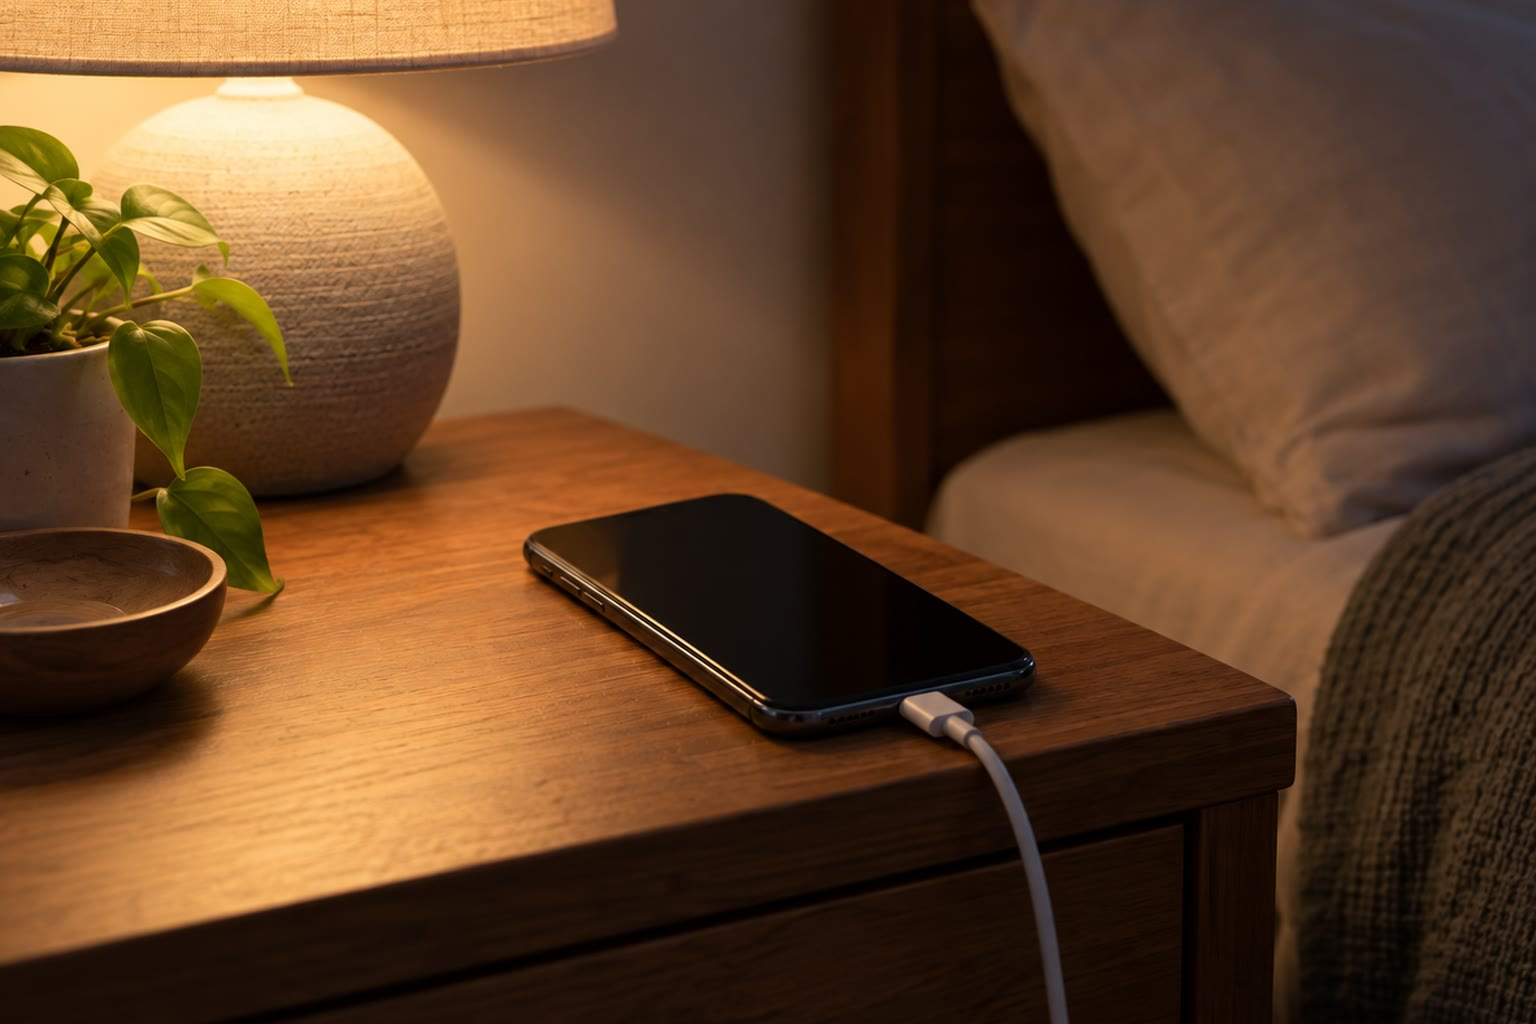
\includegraphics[width=0.45\linewidth]{images/book1/ai/g12-phone-charging.jpg}

{\small Een telefoon opladen: een reactie die 's nachts achteruit wordt
gedreven.}
\end{omfigure}

\section{Een redoxreactie in tweeën gesplitst}

Als een zinken strip in een oplossing van kopersulfaat wordt gedompeld,
wordt zink geoxideerd en worden koperionen gereduceerd aan het oppervlak
van de strip,
\ce{Zn + Cu^{2+} -> Zn^{2+} + Cu}: de \omterm{def:g9:inside-the-atom:nucleus}{elektronen} gaan direct van het
\omterm{def:g9:periodic-table-first-look:metal}{metaal} naar de \omterm{def:g9:ions:ion}{ionen}, en de energie gaat verloren als een beetje warmte.
Scheid de twee helften, en verbind ze met een draad: de \omterm{def:g9:inside-the-atom:nucleus}{elektronen} moeten
nu door de draad, en kunnen onderweg een lampje laten branden.

\begin{definition}[Elektrochemische cel, halfcel, zoutbrug]\label{def:g12:cells-and-electrolysis:cell}
Een \emph{elektrochemische cel}\index{elektrochemische cel} levert
elektrische energie uit een \omterm{def:g11:redox:reaction}{redoxreactie} waarvan de \omterm{def:g11:redox:oxidation}{oxidatie} en de
\omterm{def:g11:redox:oxidation}{reductie} in twee gescheiden compartimenten plaatsvinden. Elk compartiment,
een \omterm{def:g9:periodic-table-first-look:metal}{metalen} elektrode in een oplossing van zijn \omterm{def:g9:ions:ion}{ionen}, is een
\emph{halfcel}\index{halfcel}. Een \emph{zoutbrug}\index{zoutbrug},
een buisje of een strook papier gedrenkt in een oplossing van \omterm{def:g9:ions:ion}{ionen},
verbindt de twee oplossingen en sluit de stroomkring, terwijl ze
gescheiden blijven.
\end{definition}

\begin{definition}[Anode, kathode]\label{def:g12:cells-and-electrolysis:anode}
De elektrode waar een \omterm{def:g11:redox:oxidation}{oxidatie} plaatsvindt, is de
\emph{anode}\index{anode}; de elektrode waar een \omterm{def:g11:redox:oxidation}{reductie} plaatsvindt, is
de \emph{kathode}\index{kathode}.
\end{definition}

\begin{omfigure}
\begin{tikzpicture}[font=\small, scale=1.25]
  \pic[transform shape] at (0,0) {beaker={0.7}{black!6}};
  \pic[transform shape] at (4,0) {beaker={0.7}{cyan!70!blue!35}};
  \pic[transform shape] (zn) at (-0.3,0.25) {electrode={black!30}};
  \pic[transform shape] (cu) at (4.3,0.25) {electrode={orange!70!brown}};
  \pic[transform shape] at (0.35,0.6) {saltbridge={3.3}};
  \pic[transform shape] (v) at (2,3.9) {meter={1.10 V}};
  \draw[black!70, thick] (zn-top) |- (1.0,3.4) -| (v-a);
  \draw[black!70, thick] (cu-top) |- (3.0,3.4) -| (v-b);
  \draw[->, omProp, very thick] (0.2,3.55) -- (1.0,3.55);
  \draw[->, omProp, very thick] (3.0,3.55) -- (3.8,3.55);
  \node[omProp, font=\footnotesize] at (0.6,3.75) {$e^-$};
  \node[omProp, font=\footnotesize] at (3.4,3.75) {$e^-$};
  \node[anchor=north, align=center] at (-0.2,-0.15) {anode ($-$): zink\\ \ce{Zn -> Zn^{2+} + 2e-}};
  \node[anchor=north, align=center] at (4.2,-0.15) {kathode ($+$): koper\\ \ce{Cu^{2+} + 2e- -> Cu}};
  \node[font=\footnotesize, anchor=east, align=right] at (-0.95,0.7) {\ce{Zn^{2+}}\\ \ce{SO4^{2-}}};
  \node[font=\footnotesize, anchor=west, align=left] at (4.95,0.7) {\ce{Cu^{2+}}\\ \ce{SO4^{2-}}};
  \node[font=\footnotesize, align=center] at (2,2.45) {zoutbrug\\ (\ce{K+}, \ce{NO3-})};
\end{tikzpicture}

{\small De Daniell-cel. \omterm{def:g9:inside-the-atom:nucleus}{Elektronen} verlaten de zinken \omterm{def:g12:cells-and-electrolysis:anode}{anode} via de draad
en komen de koperen \omterm{def:g12:cells-and-electrolysis:anode}{kathode} binnen; in de \omterm{def:g12:cells-and-electrolysis:cell}{zoutbrug} bewegen \omterm{def:g9:ions:ion}{ionen} zo dat
elke oplossing neutraal blijft.}
\end{omfigure}

\begin{proposition}[Waar de elektronen heen gaan]\label{prop:g12:cells-and-electrolysis:flow}
In een cel die stroom levert, verlaten de \omterm{def:g9:inside-the-atom:nucleus}{elektronen} de cel via de \omterm{def:g12:cells-and-electrolysis:anode}{anode},
waar ze bij de \omterm{def:g11:redox:oxidation}{oxidatie} vrijkomen, gaan ze door de uitwendige
stroomkring, en komen ze binnen via de \omterm{def:g12:cells-and-electrolysis:anode}{kathode}, waar de \omterm{def:g11:redox:oxidation}{reductie} ze
opneemt. De \omterm{def:g12:cells-and-electrolysis:anode}{anode} is de negatieve pool, de \omterm{def:g12:cells-and-electrolysis:anode}{kathode} de positieve. Binnenin
wordt de stroom gedragen door \omterm{def:g9:ions:ion}{ionen}: \omterm{def:g9:ions:ion}{kationen} bewegen naar de \omterm{def:g12:cells-and-electrolysis:anode}{kathode},
\omterm{def:g9:ions:ion}{anionen} naar de \omterm{def:g12:cells-and-electrolysis:anode}{anode}.
\end{proposition}

\begin{proof}
De \omterm{def:g11:redox:oxidation}{oxidatie} levert \omterm{def:g9:inside-the-atom:nucleus}{elektronen} aan de \omterm{def:g12:cells-and-electrolysis:anode}{anode}; de \omterm{def:g11:redox:oxidation}{reductie} verbruikt ze aan
de \omterm{def:g12:cells-and-electrolysis:anode}{kathode}; de draad is de enige weg tussen die twee. Anders zou elke
oplossing geladen raken, en dat voorkomen de \omterm{def:g9:ions:ion}{ionen} van de \omterm{def:g12:cells-and-electrolysis:cell}{zoutbrug}.
\end{proof}

\begin{method}[Een cel beschrijven]\label{met:g12:cells-and-electrolysis:describe}
\begin{enumerate}
  \item Schrijf de totale \omterm{def:g11:redox:reaction}{redoxreactie} op die vanzelf verloopt.
  \item Splits haar in twee \omterm{def:g11:redox:couple}{halfreacties}: de \omterm{def:g11:redox:oxidation}{oxidatie} (\omterm{def:g12:cells-and-electrolysis:anode}{anode}) en de
        \omterm{def:g11:redox:oxidation}{reductie} (\omterm{def:g12:cells-and-electrolysis:anode}{kathode}).
  \item Geef de polariteit aan: \omterm{def:g12:cells-and-electrolysis:anode}{anode} $-$, \omterm{def:g12:cells-and-electrolysis:anode}{kathode} $+$; de richting van de
        \omterm{def:g9:inside-the-atom:nucleus}{elektronen} in de draad (van \omterm{def:g12:cells-and-electrolysis:anode}{anode} naar \omterm{def:g12:cells-and-electrolysis:anode}{kathode}) en van de stroom
        (van \omterm{def:g12:cells-and-electrolysis:anode}{kathode} naar \omterm{def:g12:cells-and-electrolysis:anode}{anode}).
  \item Beschrijf de beweging van de \omterm{def:g9:ions:ion}{ionen} in de \omterm{def:g12:cells-and-electrolysis:cell}{zoutbrug}.
\end{enumerate}
\end{method}


\begin{history}[De zuil van Volta, 1800]
In 1800 stapelde de natuurkundige Alessandro Volta schijfjes van twee
verschillende \omterm{def:g9:periodic-table-first-look:metal}{metalen}, zink en koper of zilver, gescheiden door lapjes
stof gedrenkt in pekel, en kreeg zo een constante elektrische stroom: de
eerste batterij. Ze gaf natuurkundigen hun eerste continue bron van
elektriciteit, en scheikundigen een nieuw werktuig: binnen een paar jaar
had \omterm{def:g12:cells-and-electrolysis:electrolysis}{elektrolyse} voor het eerst natrium en kalium geïsoleerd.
\end{history}

\begin{omfigure}
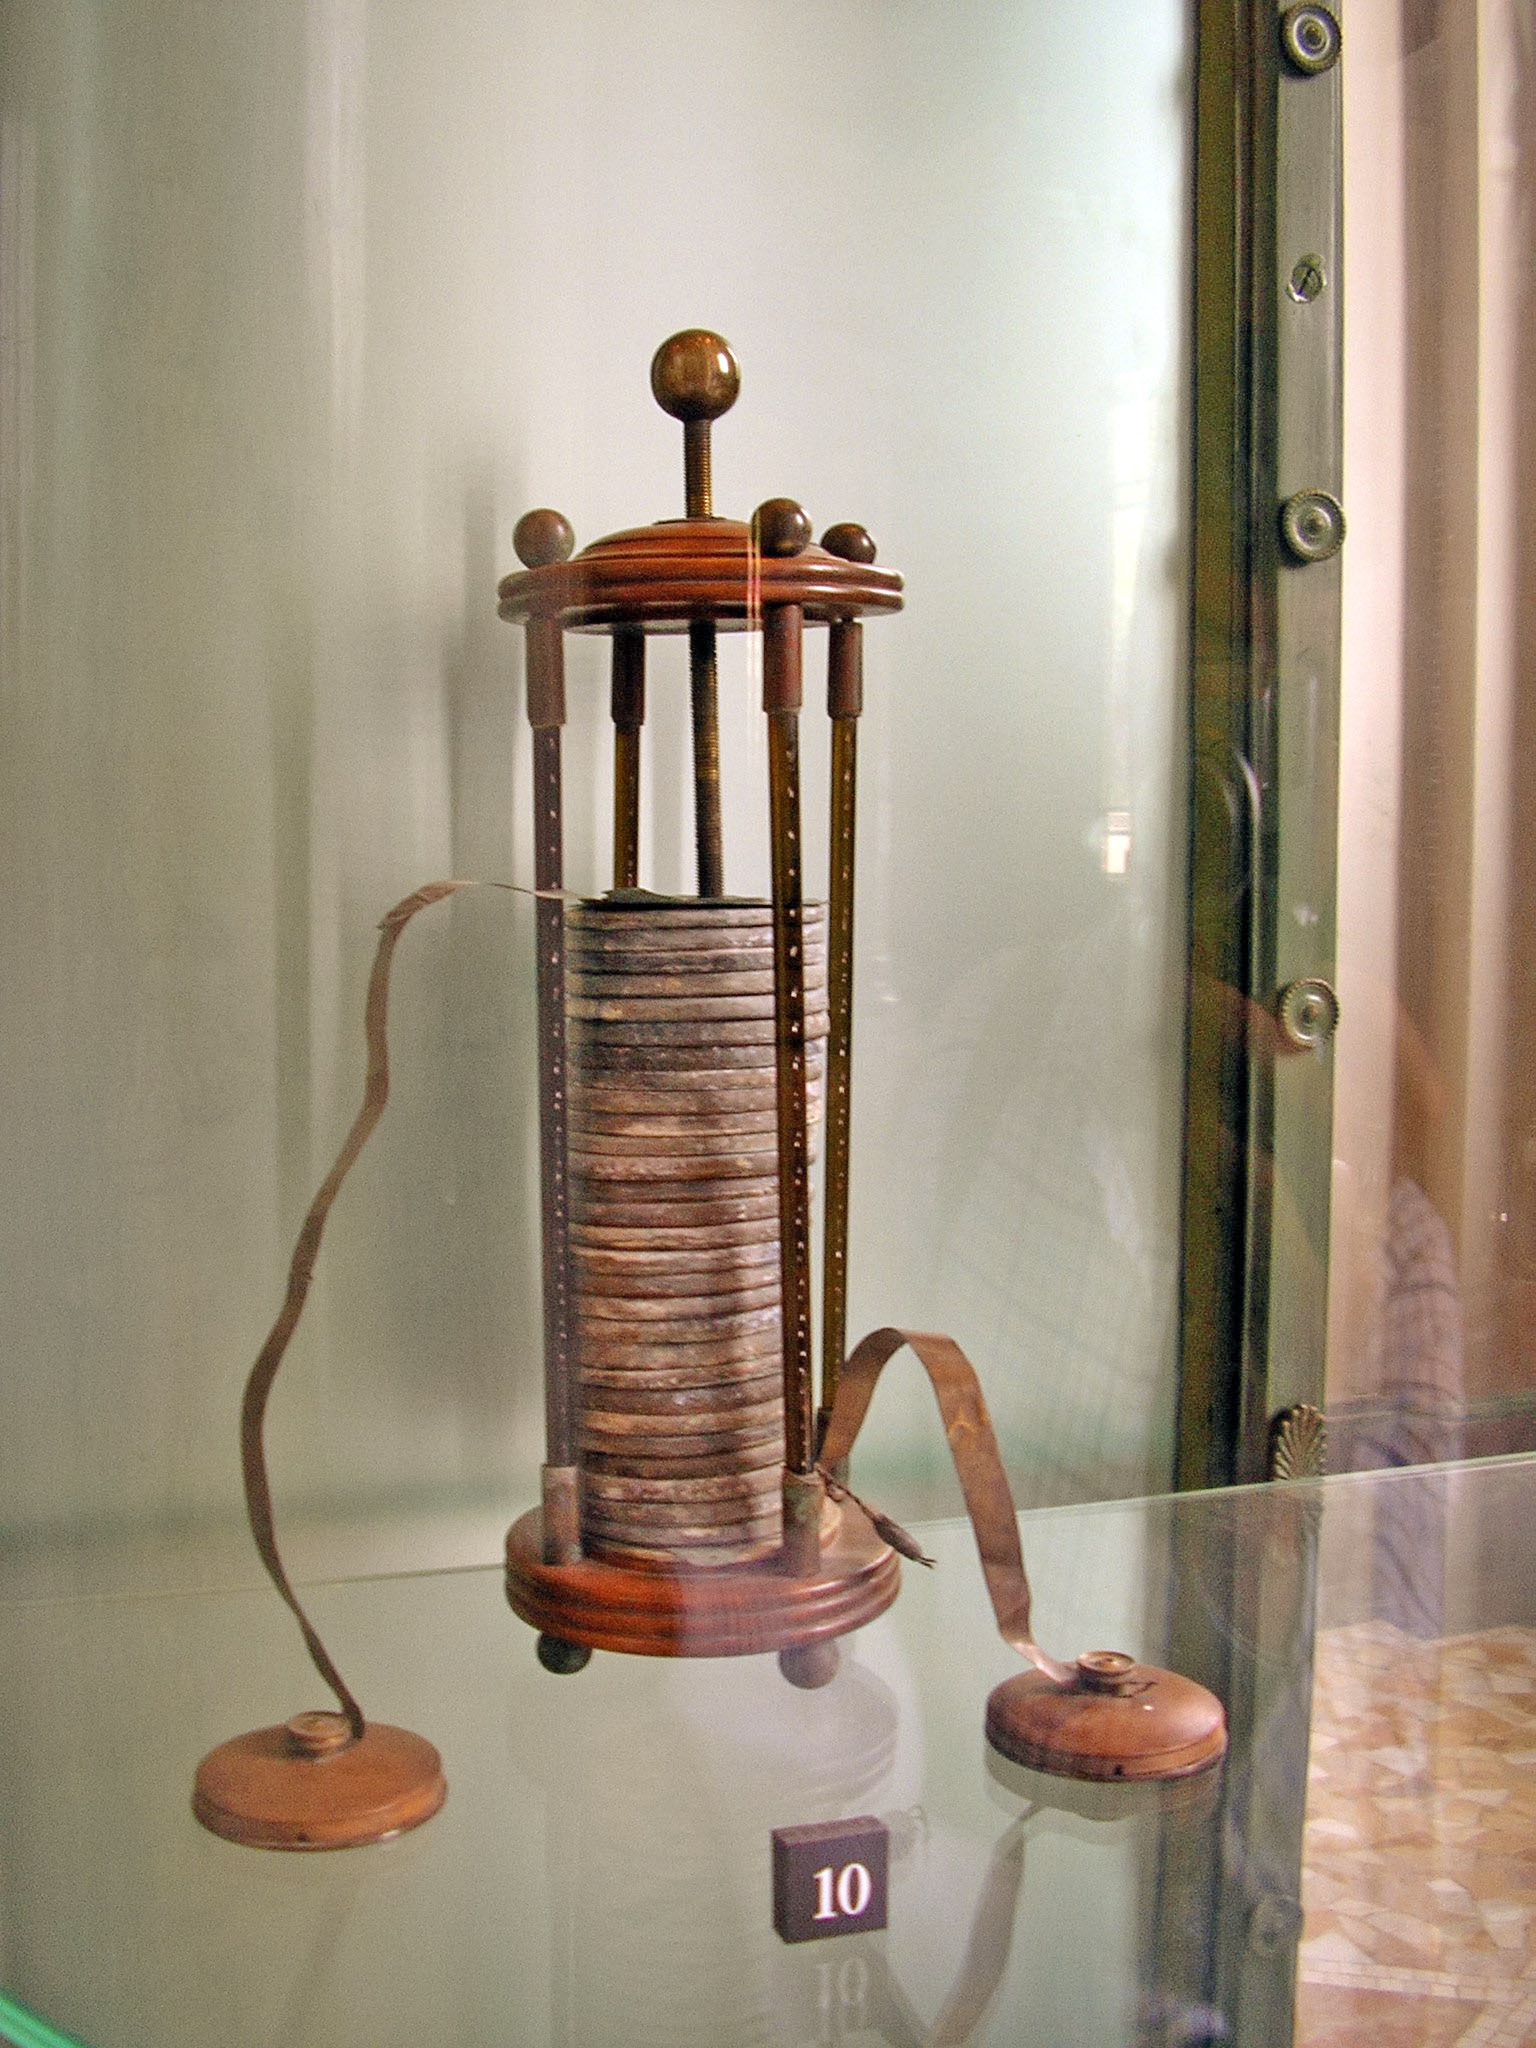
\includegraphics[width=0.24\linewidth]{images/book1/volta-pile.jpg}

{\small Een zuil van Volta in een museum. Foto GuidoB, CC BY-SA 3.0.}
\end{omfigure}

\section{De spanning van een cel}

\begin{definition}[Celspanning]\label{def:g12:cells-and-electrolysis:emf}
De \emph{celspanning}\index{celspanning} is de spanning die met een
voltmeter gemeten wordt tussen de polen van een cel die geen stroom
levert (open stroomkring); ze is positief als de plus van de voltmeter op
de \omterm{def:g12:cells-and-electrolysis:anode}{kathode} zit.
\end{definition}

\begin{example}[De Daniell-cel]\label{ex:g12:cells-and-electrolysis:daniell}
% ledger: e0:Cu, e0:Zn, emf:Daniell
Met beide oplossingen op \qty{1}{mol/L} geeft de Daniell-cel
\qty{1.10}{V}. Hoe je zo'n spanning voorspelt met tabellen van
elektrodepotentialen, laat het deel voor het eerste universiteitsjaar
zien.
\end{example}

\begin{remark}[Waarom een cel leegraakt]\label{rem:g12:cells-and-electrolysis:runs-down}
De reactie van de cel, \ce{Zn + Cu^{2+} -> Zn^{2+} + Cu}, heeft een heel
grote constante $K$. Terwijl de cel werkt, neemt
$Q = [\ce{Zn^{2+}}]/[\ce{Cu^{2+}}]$ toe, en de reactie blijft lopen zolang
$Q < K$. Als een \omterm{def:g7:chemical-reactions:reactant}{beginstof} op is (het zink, of de koperionen), stopt de
stroom: de cel is ``leeg''.
\end{remark}

\section{Lading en capaciteit}

\begin{definition}[Constante van Faraday, capaciteit]\label{def:g12:cells-and-electrolysis:capacity}
De \emph{constante van Faraday}\index{constante van Faraday} $F$ is de
elektrische lading van één \omterm{def:g10:the-mole:amount}{mol} \omterm{def:g9:inside-the-atom:nucleus}{elektronen},
$F = N_A e = \qty{96485}{C/mol}$. De
\emph{capaciteit}\index{capaciteit} van een cel is de grootste elektrische
lading die ze kan leveren, vaak opgegeven in ampère-uur:
$\qty{1}{A.h} = \qty{3600}{C}$.
\end{definition}

\begin{proposition}[Lading en hoeveelheid elektronen]\label{prop:g12:cells-and-electrolysis:charge}
% ledger: const:F, const:NA, const:e
Een stroom $I$ die gedurende een tijd $\Delta t$ loopt, voert de lading
$Q = I\,\Delta t$ mee, dat is een hoeveelheid \omterm{def:g9:inside-the-atom:nucleus}{elektronen}
\[
  n(e^-) = \frac{Q}{F} = \frac{I\,\Delta t}{F} .
\]
\end{proposition}

\begin{proof}
Elk \omterm{def:g9:inside-the-atom:nucleus}{elektron} draagt de elementaire lading $e$; $n$ \omterm{def:g10:the-mole:amount}{mol} \omterm{def:g9:inside-the-atom:nucleus}{elektronen} dragen
$n N_A e = n F$.
\end{proof}

\begin{example}[Capaciteit van een Daniell-cel]\label{ex:g12:cells-and-electrolysis:capacity}
% ledger: aw:Zn, const:F
De zinkelektrode bevat \qty{6.5}{g} zink dat kan reageren, dat is
$6.5/65.4 = \qty{0.099}{mol}$. Elk zinkatoom geeft twee \omterm{def:g9:inside-the-atom:nucleus}{elektronen}:
$n(e^-) = \qty{0.199}{mol}$, dus $Q = 0.199 \times 96485 = \qty{1.9e4}{C}$,
ongeveer $\qty{1.9e4}{}/3600 = \qty{5.3}{A.h}$, als de koperionen niet
eerder opraken.
\end{example}

\section{Elektrolyse}

\begin{definition}[Elektrolyse, accu]\label{def:g12:cells-and-electrolysis:electrolysis}
Een \emph{elektrolyse}\index{elektrolyse} is een \omterm{def:g11:redox:reaction}{redoxreactie} die door
een elektrische spanningsbron wordt afgedwongen, in de richting
tegengesteld aan die welke ze uit zichzelf zou nemen. Een
\emph{accu}\index{accu} is een cel die je kunt opladen: tijdens het
opladen drijft de spanningsbron haar reactie achteruit, als een
elektrolyse.
\end{definition}

\begin{inthelab}[Elektrolyse van water]
Twee elektroden staan in water dat geleidend is gemaakt met een beetje
natriumsulfaat, elk onder een omgekeerde reageerbuis vol oplossing. Met
een spanningsbron van een paar volt stijgen er belletjes op bij beide
elektroden: bij de \omterm{def:g12:cells-and-electrolysis:anode}{kathode} (verbonden met de $-$-pool) waterstof, bij de
\omterm{def:g12:cells-and-electrolysis:anode}{anode} zuurstof, twee keer zoveel van het eerste als van het tweede. Een
brandende spaander geeft in het eerste gas een plofje; een gloeiende
spaander vlamt in het tweede weer op.
\end{inthelab}

\begin{omfigure}
\begin{tikzpicture}[font=\small, scale=1.2]
  % een bak water met twee omgekeerde buizen erin
  \fill[omWater] (-1.4,0) rectangle (1.4,1.1);
  \foreach \x/\g in {-0.6/1.2, 0.6/0.6} {
    \fill[omWater] (\x-0.18,0.3) rectangle (\x+0.18,2.9);
    \fill[white] (\x-0.18,{2.9-\g}) rectangle (\x+0.18,2.9);
    \fill[white] (\x,2.9) circle (0.18);
    \draw[om glass] (\x-0.18,0.3) -- (\x-0.18,2.9) arc[start angle=180, end angle=0, radius=0.18] -- (\x+0.18,0.3);
  }
  \draw[om glass] (-1.5,1.25) -- (-1.4,1.15) -- (-1.4,0) -- (1.4,0) -- (1.4,1.15) -- (1.5,1.25);
  \fill[black!55] (-0.65,0) rectangle (-0.55,0.6);
  \fill[black!55] (0.55,0) rectangle (0.65,0.6);
  \node[draw, fill=white, minimum width=1.6cm, minimum height=0.45cm, font=\footnotesize] (g) at (0,-0.75) {spanningsbron};
  \draw[black!70, thick] (-0.6,0) -- (-0.6,0 |- g.north);
  \draw[black!70, thick] (0.6,0) -- (0.6,0 |- g.north);
  \node[font=\footnotesize] at (-0.78,-0.3) {$-$};
  \node[font=\footnotesize] at (0.78,-0.3) {$+$};
  \node[anchor=east, align=right] at (-0.95,2.5) {waterstof\\ (kathode)};
  \node[anchor=west, align=left] at (0.95,2.5) {zuurstof\\ (anode)};
\end{tikzpicture}

{\small \omterm{def:g12:cells-and-electrolysis:electrolysis}{Elektrolyse} van water: boven de elektroden verzamelt zich twee
keer zoveel waterstof als zuurstof.}
\end{omfigure}


\begin{example}[Water, gesplitst]\label{ex:g12:cells-and-electrolysis:water}
Aan de \omterm{def:g12:cells-and-electrolysis:anode}{kathode}: \ce{2H2O + 2e- -> H2 + 2OH-}; aan de \omterm{def:g12:cells-and-electrolysis:anode}{anode}:
\ce{6H2O -> O2 + 4H3O+ + 4e-}. Voor vier \omterm{def:g9:inside-the-atom:nucleus}{elektronen} ontstaan twee
\omterm{def:g7:atoms-and-molecules:molecule}{moleculen} waterstof en één \omterm{def:g7:atoms-and-molecules:molecule}{molecuul} zuurstof, terwijl de \omterm{def:g9:ions:ion}{ionen} \ce{H3O+}
en \ce{OH-} die aan de twee elektroden ontstaan, weer water vormen:
totaal \ce{2H2O -> 2H2 + O2}, het
omgekeerde van de \omterm{def:g4:what-a-fire-needs:burning}{verbranding} van waterstof, waarvoor energie nodig is.
\end{example}

\begin{method}[Massa die bij een elektrolyse neerslaat]\label{met:g12:cells-and-electrolysis:mass}
\begin{enumerate}
  \item Schrijf de \omterm{def:g11:redox:couple}{halfreactie} op aan de elektrode waar het \omterm{def:g9:periodic-table-first-look:metal}{metaal}
        ontstaat, bijvoorbeeld \ce{Cu^{2+} + 2e- -> Cu}.
  \item Bereken de lading $Q = I \Delta t$ en $n(e^-) = Q/F$.
  \item Deel door het aantal \omterm{def:g9:inside-the-atom:nucleus}{elektronen} per \omterm{def:g7:atoms-and-molecules:atom}{atoom}: $n(\ce{Cu}) =
        n(e^-)/2$; daarna $m = n \times M$.
\end{enumerate}
\end{method}


\begin{example}[Koper raffineren]\label{ex:g12:cells-and-electrolysis:refining}
% ledger: aw:Cu, const:F
Onzuiver koper uit de smelterij wordt de \omterm{def:g12:cells-and-electrolysis:anode}{anode} van een elektrolysecel in
een oplossing van kopersulfaat, en een dun plaatje zuiver koper de
\omterm{def:g12:cells-and-electrolysis:anode}{kathode}. Aan de \omterm{def:g12:cells-and-electrolysis:anode}{anode} lost koper op, \ce{Cu -> Cu^{2+} + 2e-}; aan de
\omterm{def:g12:cells-and-electrolysis:anode}{kathode} slaat zuiver koper neer, \ce{Cu^{2+} + 2e- -> Cu}; de
verontreinigingen zakken naar de bodem of blijven in oplossing. Een
stroom van \qty{100}{A} gedurende
\qty{24}{h} voert $Q = 100 \times 86400 = \qty{8.64e6}{C}$ mee, dat is
$n(e^-) = \qty{89.5}{mol}$, waarmee $89.5/2 = \qty{44.8}{mol}$ koper
neerslaat: \qty{2.84}{kg}.
\end{example}

\begin{omfigure}
\begin{tikzpicture}[font=\small, scale=1.25]
  \pic[transform shape] at (0,0) {beaker={0.75}{cyan!70!blue!35}};
  \pic[transform shape] (an) at (-0.4,0.2) {electrode={orange!40!brown!80!black}};
  \pic[transform shape] (ca) at (0.4,0.2) {electrode={orange!80!brown}};
  \foreach \p in {(-0.6,0.08),(-0.5,0.12),(-0.3,0.07),(-0.2,0.1)} \fill[black!55] \p circle (0.03);
  \node[draw, fill=white, font=\footnotesize, minimum width=1.6cm] (g) at (0,3.4) {spanningsbron};
  \draw[black!70, thick] (an-top) -- (an-top |- g.south);
  \draw[black!70, thick] (ca-top) -- (ca-top |- g.south);
  \node[font=\footnotesize] at (-0.58,2.95) {$+$};
  \node[font=\footnotesize] at (0.58,2.95) {$-$};
  \draw[omProp, thick, <-] (-0.55,1.2) -- (-1.6,1.6) node[left, align=right, text=black] {onzuiver koper\\ anode: lost op};
  \draw[omProp, thick, <-] (0.55,1.2) -- (1.6,1.6) node[right, align=left, text=black] {zuiver koper\\ kathode: groeit};
  \draw[omProp, thick, <-] (-0.35,0.1) -- (-1.6,0.3) node[left, text=black] {verontreinigingen};
\end{tikzpicture}

{\small Koper raffineren door \omterm{def:g12:cells-and-electrolysis:electrolysis}{elektrolyse}: koper gaat via de oplossing van
de onzuivere \omterm{def:g12:cells-and-electrolysis:anode}{anode} naar de zuivere \omterm{def:g12:cells-and-electrolysis:anode}{kathode}.}
\end{omfigure}

\section{Batterijen, accu's en brandstofcellen}

Elke batterij is een cel, elke oplaadbare batterij een \omterm{def:g12:cells-and-electrolysis:electrolysis}{accu}. De loodaccu
van een auto werkt met lood, loodoxide en zwavelzuur; de
lithiumionaccu van een telefoon verplaatst lithiumionen tussen twee
elektroden, een van grafiet en een van een metaaloxide, door een vloeibare
elektrolyt of een polymeerelektrolyt, terwijl de \omterm{def:g9:inside-the-atom:nucleus}{elektronen} via de
uitwendige stroomkring rondgaan. Een brandstofcel is een cel waarvan de
\omterm{def:g7:chemical-reactions:reactant}{beginstoffen} voortdurend worden aangevoerd:
een waterstofbrandstofcel laat de reactie \ce{2H2 + O2 -> 2H2O} verlopen,
het omgekeerde van de \omterm{def:g12:cells-and-electrolysis:electrolysis}{elektrolyse} van water, en levert elektriciteit en
water. Waterstof die door \omterm{def:g12:cells-and-electrolysis:electrolysis}{elektrolyse} met elektriciteit uit wind of zon
wordt gemaakt en daarna in brandstofcellen wordt gebruikt, is een manier
om die elektriciteit op te slaan.

\begin{omfigure}
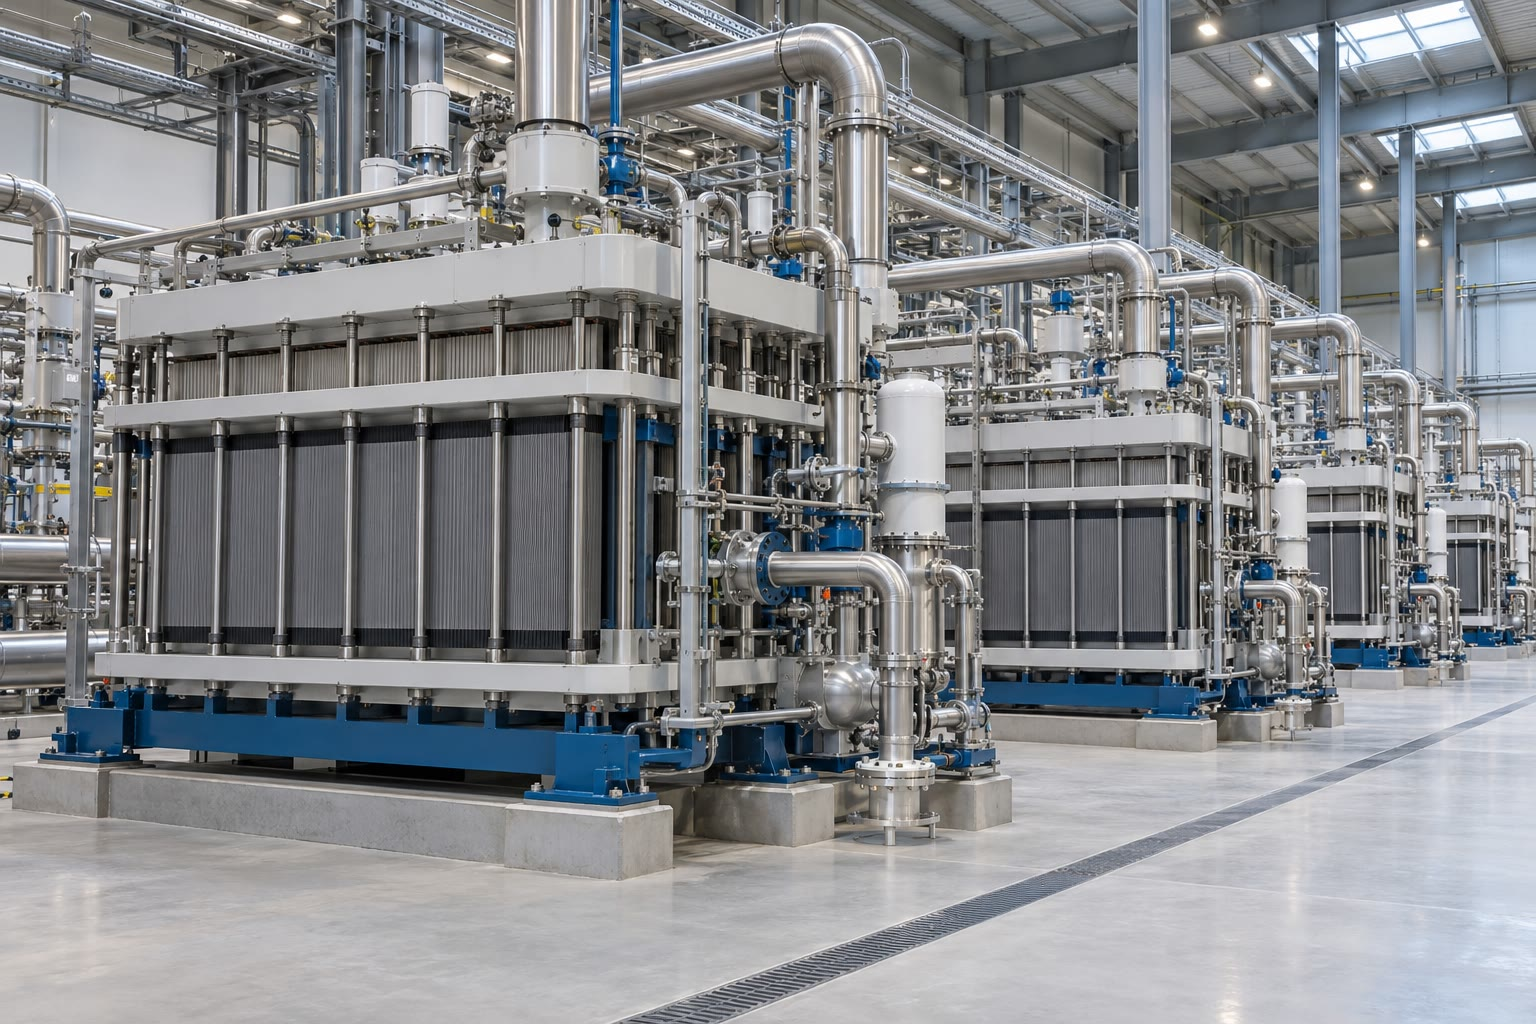
\includegraphics[width=0.48\linewidth]{images/book1/ai/g12-electrolyser-hall.jpg}

{\small Een hal met elektrolysers: water wordt gesplitst in waterstof en
zuurstof.}
\end{omfigure}

\section{Oefeningen}

\begin{exercise}[$\star$]\label{exo:g12:cells-and-electrolysis:1}
Welke elektrode is in de Daniell-cel de \omterm{def:g12:cells-and-electrolysis:anode}{anode}? En de \omterm{def:g12:cells-and-electrolysis:anode}{kathode}? Schrijf
bij elk de \omterm{def:g11:redox:couple}{halfreactie} op.
\end{exercise}

\begin{exercise}[$\star$]\label{exo:g12:cells-and-electrolysis:2}
Een stroom van \qty{0.20}{A} loopt gedurende \qty{30}{min}. Bereken de
lading die meegevoerd wordt en de hoeveelheid \omterm{def:g9:inside-the-atom:nucleus}{elektronen}.
\end{exercise}

\begin{exercise}[$\star$]\label{exo:g12:cells-and-electrolysis:3}
Wat is de rol van de \omterm{def:g12:cells-and-electrolysis:cell}{zoutbrug}? Wat gebeurt er als je haar weghaalt?
\end{exercise}

\begin{exercise}[$\star$]\label{exo:g12:cells-and-electrolysis:4}
Reken een \omterm{def:g12:cells-and-electrolysis:capacity}{capaciteit} van \qty{2.5}{A.h} om in coulomb.
\end{exercise}

\begin{exercise}[$\star$]\label{exo:g12:cells-and-electrolysis:5}
Verloopt de reactie bij een \omterm{def:g12:cells-and-electrolysis:electrolysis}{elektrolyse} vanzelf? Wat levert de energie?
\end{exercise}

\begin{exercise}[$\star\star$]\label{exo:g12:cells-and-electrolysis:6}
Een cel bestaat uit een zilverelektrode in zilvernitraat en een
koperelektrode in kopersulfaat. De voltmeter laat zien dat de \omterm{def:g9:inside-the-atom:nucleus}{elektronen}
via het koper vertrekken. Schrijf de \omterm{def:g11:redox:couple}{halfreacties} op, benoem de \omterm{def:g12:cells-and-electrolysis:anode}{anode} en
de \omterm{def:g12:cells-and-electrolysis:anode}{kathode}, en geef de totale reactie.
\end{exercise}

\begin{exercise}[$\star\star$]\label{exo:g12:cells-and-electrolysis:7}
Een horlogebatterij levert drie jaar lang voortdurend \qty{10}{\micro A}.
Wat is haar \omterm{def:g12:cells-and-electrolysis:capacity}{capaciteit} in \si{mA.h}?
\end{exercise}

\begin{exercise}[$\star\star$]\label{exo:g12:cells-and-electrolysis:8}
Een lepel wordt verzilverd met een stroom van \qty{0.50}{A} gedurende
\qty{40}{min}, \ce{Ag+ + e- -> Ag}. Welke massa zilver slaat er neer?
\end{exercise}

\begin{exercise}[$\star\star$]\label{exo:g12:cells-and-electrolysis:9}
Geef in de figuur van de Daniell-cel de richting van de stroom in de
draad, en de richting waarin de \omterm{def:g9:ions:ion}{ionen} \ce{K+} en \ce{NO3-} van de
\omterm{def:g12:cells-and-electrolysis:cell}{zoutbrug} bewegen.
\end{exercise}

\begin{exercise}[$\star\star$]\label{exo:g12:cells-and-electrolysis:10}
Vergelijk een cel en een \omterm{def:g12:cells-and-electrolysis:electrolysis}{elektrolyse}: het teken van de \omterm{def:g12:cells-and-electrolysis:anode}{anode}, de richting
van de reactie, de omzetting van energie.
\end{exercise}

\begin{exercise}[$\star\star$]\label{exo:g12:cells-and-electrolysis:11}
Bij de \omterm{def:g12:cells-and-electrolysis:electrolysis}{elektrolyse} van water wordt \qty{24}{mL} waterstof opgevangen.
Welk volume zuurstof wordt er tegelijk opgevangen? Waarom?
\end{exercise}

\begin{exercise}[$\star\star\star$]\label{exo:g12:cells-and-electrolysis:12}
Een Daniell-cel bevat \qty{5.0}{g} zink en \qty{100}{mL} kopersulfaat van
\qty{0.50}{mol/L}. Welke \omterm{def:g7:chemical-reactions:reactant}{beginstof} raakt het eerst op? Wat is de
\omterm{def:g12:cells-and-electrolysis:capacity}{capaciteit} van de cel? Hoe lang kan ze \qty{50}{mA} leveren?
\end{exercise}

\begin{exercise}[$\star\star\star$]\label{exo:g12:cells-and-electrolysis:13}
Een batterij van \qty{1.5}{V} levert \qty{2.0}{A.h}. Bereken de energie
die ze opslaat ($E = Q U$), in joule en in wattuur.
\end{exercise}

\begin{exercise}[$\star\star\star$]\label{exo:g12:cells-and-electrolysis:14}
Water wordt gedurende \qty{1.0}{h} geëlektrolyseerd met \qty{2.0}{A}.
Bereken de hoeveelheden, en daarna de volumes bij \qty{20}{\celsius}
($V_m = \qty{24.1}{L/mol}$), van de waterstof en de zuurstof die
ontstaan.
\end{exercise}

\begin{exercise}[$\star\star\star$]\label{exo:g12:cells-and-electrolysis:15}
Bij het raffineren van koper verliest de \omterm{def:g12:cells-and-electrolysis:anode}{anode} \qty{3.00}{kg} materiaal,
terwijl de \omterm{def:g12:cells-and-electrolysis:anode}{kathode} \qty{2.84}{kg} koper wint. Wat is het
koperpercentage van de onzuivere \omterm{def:g12:cells-and-electrolysis:anode}{anode}, als je aanneemt dat aan de \omterm{def:g12:cells-and-electrolysis:anode}{anode}
alleen koper geoxideerd wordt en dat de verontreinigingen er gewoon
afvallen?
\end{exercise}

\section{Probleem: De telefoonaccu}

\begin{problem}[{Weekendprobleem --- welke massa lithium pendelt er tussen
de elektroden van een telefoonaccu van \qty{4000}{mA.h}?}]
\label{pb:g12:cells-and-electrolysis:1}
% ledger: const:F, const:NA, aw:Li, dch:CH4, aw:C, aw:H
Op een telefoonaccu staat ``\qty{3.7}{V}, \qty{4000}{mA.h}''. In een
vereenvoudigd beeld geeft tijdens het ontladen elk lithiumatoom dat in de
grafietelektrode is opgeslagen één \omterm{def:g9:inside-the-atom:nucleus}{elektron} af en vertrekt het als
lithiumion,
\ce{Li -> Li+ + e-}; het \omterm{def:g9:ions:ion}{ion} steekt de elektrolyt over en wordt opgenomen
door de metaaloxide-elektrode, die tegelijk een \omterm{def:g9:inside-the-atom:nucleus}{elektron} opneemt.

\medskip
\noindent\textbf{Deel I --- De cel.}
\begin{enumerate}
  \item Is de grafietelektrode tijdens het ontladen de \omterm{def:g12:cells-and-electrolysis:anode}{anode} of de
        \omterm{def:g12:cells-and-electrolysis:anode}{kathode}? Waarom?
  \item Welke elektrode is de negatieve pool?
  \item In welke richting gaan de \omterm{def:g9:inside-the-atom:nucleus}{elektronen} door de telefoon? En de
        lithiumionen in de \omterm{def:g12:cells-and-electrolysis:electrolysis}{accu}?
  \item Waarom is deze cel een \omterm{def:g12:cells-and-electrolysis:electrolysis}{accu}?
\end{enumerate}

\medskip
\noindent\textbf{Deel II --- De lading.}
\begin{enumerate}[resume]
  \item Reken \qty{4000}{mA.h} om in ampère-uur, en daarna in coulomb.
  \item Bereken de hoeveelheid \omterm{def:g9:inside-the-atom:nucleus}{elektronen} die deze lading voorstelt.
  \item Hoeveel \omterm{def:g9:inside-the-atom:nucleus}{elektronen} zijn dat?
  \item De telefoon gebruikt gemiddeld \qty{0.25}{A}. Hoe lang gaat een
        volle \omterm{def:g12:cells-and-electrolysis:electrolysis}{accu} mee?
  \item Het scherm geeft 20 \% aan. Welke lading, in coulomb, is er nog
        over?
\end{enumerate}

\medskip
\noindent\textbf{Deel III --- De energie.}
\begin{enumerate}[resume]
  \item Bereken de opgeslagen energie, $E = Q U$, in joule.
  \item Reken die om in wattuur.
  \item Vergelijk met de energie die vrijkomt bij de \omterm{def:g4:what-a-fire-needs:burning}{verbranding} van
        \qty{1}{g} methaan (\qty{55.7}{kJ}).
  \item Hoeveel volledige oplaadbeurten levert \qty{1}{kW.h} elektriciteit,
        als er geen energie verloren zou gaan?
\end{enumerate}

\medskip
\noindent\textbf{Deel IV --- Opladen.}
\begin{enumerate}[resume]
  \item Welke reactie vindt tijdens het opladen plaats aan de
        grafietelektrode? Is het een \omterm{def:g11:redox:oxidation}{oxidatie} of een \omterm{def:g11:redox:oxidation}{reductie}?
  \item Waarom is opladen een \omterm{def:g12:cells-and-electrolysis:electrolysis}{elektrolyse}?
  \item De lader levert \qty{2.0}{A}. Hoe lang duurt een volledige
        oplaadbeurt minstens?
  \item Welke hoeveelheid lithiumionen steekt tijdens één volledige
        oplaadbeurt de elektrolyt over?
  \item Bereken hun massa.
  \item Geef het eindantwoord: welke massa lithium pendelt er bij één
        volledige oplaadbeurt tussen de elektroden?
\end{enumerate}
\end{problem}
